%%%%%%%%%%%%%%%%%%%%%%%%%%%%%%%%%%%%%%%%%%%%%%
%                insertmeeting
% 1) Title (something creative & funny?)
% 2) Date (MM/DD/YYYY)
% 3) Location (ex. Hagerty High School)
% 4) People/Committees Present 
% 5) Picture 
% 6) Start Time & Stop Time (ex. 12:30AM to 4:30PM)
%%%%%%%%%%%%%%%%%%%%%%%%%%%%%%%%%%%%%%%%%%%%%%
\insertmeeting 
	{Summer Camp Craze!} 
	{08/31/21}
	{Hagerty High School}
	{Annika, Jensen, Nathan, Ritam, Samantha}
	{Images/RobotPics/robot.jpg}
	{9:00 - 2:00}
	
\hhscommittee{Outreach}
\noindent\hfil\rule{\textwidth}{.4pt}\hfil
\subsubsection*{Goals}
\begin{itemize}
    \item Introduce potential incoming members to the hagerty robotics program
    \item Build Potential members' interest in robotics

\end{itemize} 

\noindent\hfil\rule{\textwidth}{.4pt}\hfil

\subsubsection*{Accomplishments}
As a program, Hagerty robotics planned and held a 4 day summer camp to help bring aspiring members into our program and teach them about FIRST and VEX robotics. Before the recruitment camp started, we came up with an overall plan, including several presentations about hardware, software, outreach, notebook, and multimedia. In addition to the presentations, we decided the best way for the campers to experience what robotics has to offer was to hold a mini competition based on summer camps we have held in the past. This competition had the campers build a robot, create an autonomous program and write an engineering notebook with help from our experienced team members. When the camp started, we divided the 11 campers into 4 smaller teams; 2 FTC and 2 VEX. Inside these teams, the campers got to experience what it is like to be part of the Hagerty robotics program and were able to gain experience and knowledge from the current members of the program. At the end of the camp, we held robot matches based on real FTC and VEX meets, utilizing an original minigame, named “purpole”, that the campers had spent the previous 3 days of the camp preparing for. Overall, the camp was very successful in building the campers’ interest in the FIRST and VEX competitions, and many of them signed up to become members of the Hagerty robotics program in the upcoming season.

\hhscommittee{Hardware}
\noindent\hfil\rule{\textwidth}{.4pt}\hfil
\subsubsection*{Goals}
\begin{itemize}
    \item Help newer members learn onshape’s custom features and assemblies
  

\end{itemize} 

\noindent\hfil\rule{\textwidth}{.4pt}\hfil

\subsubsection*{Accomplishments}
At the meeting today, we wanted to work on expanding some of our newer member’s knowledge of CAD. Because we want our members to have some experience in every skill that we use, we thought now, before the game is revealed, would be the best time to start learning CAD. Because the two members that we were working with today had already learned how to make sketches, we wanted to focus more on using custom features and creating an assembly. We decided to have them follow along with one of our older Hardware committee members who would show them how to make a wood box with box joints and t-slot joints. We started out by downloading the box joint and t-slot joint custom features. From there, we had them sketch and extrude the first 3 sides of the box without any box joints or t-slot joints. After that, we showed the learning members the mirror tool, using it to mirror two of the sides of the box so that we had a 5 sided box. We finished up all of the box’s parts by adding box joints and t-slot joints into the plates, just like we do on our robot’s parts. 
From there, we created an assembly where the newer members were shown how the fasten mate works by putting the parts of the box together. Although the box still looked the same as in the part studio, mating parts together in assemblies is a very important part of CAD. To add to this knowledge, we showed them how to insert standard content, like 6-32 screws into their CAD. Although we ran out of time to show the other types of mates, we were able to cover the fasten mate well, which is the most commonly used type of mate. Overall the newer members’ CAD skills have been progressing very quickly, and they seem well equipped for the upcoming season. Next is to continue teaching less experienced CAD members other types of mates
and demonstrating more complicated skeletons. 


\begin{figure}[ht]
\centering
\begin{minipage}[b]{.48\textwidth}
  \centering
  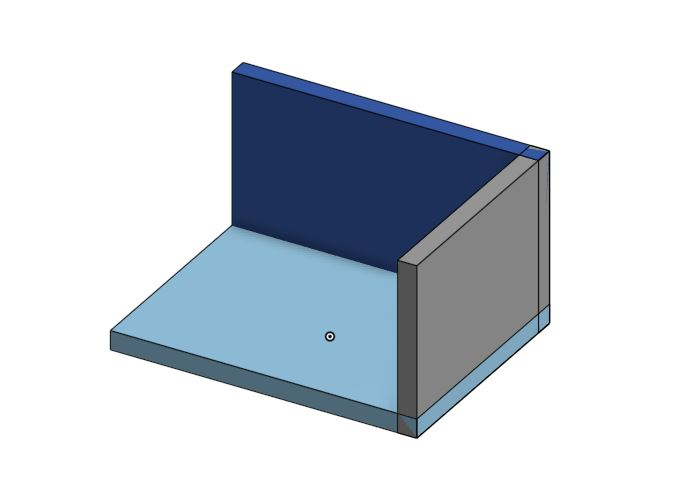
\includegraphics[width=0.95\textwidth]{Meetings/August/08-31-21/8-31-21_CAD_Image1 - Nathan Forrer.JPG}
  \caption{Three sides of the box}
  \label{fig:083121_1}
\end{minipage}%
\hfill%
\begin{minipage}[b]{.48\textwidth}
  \centering
  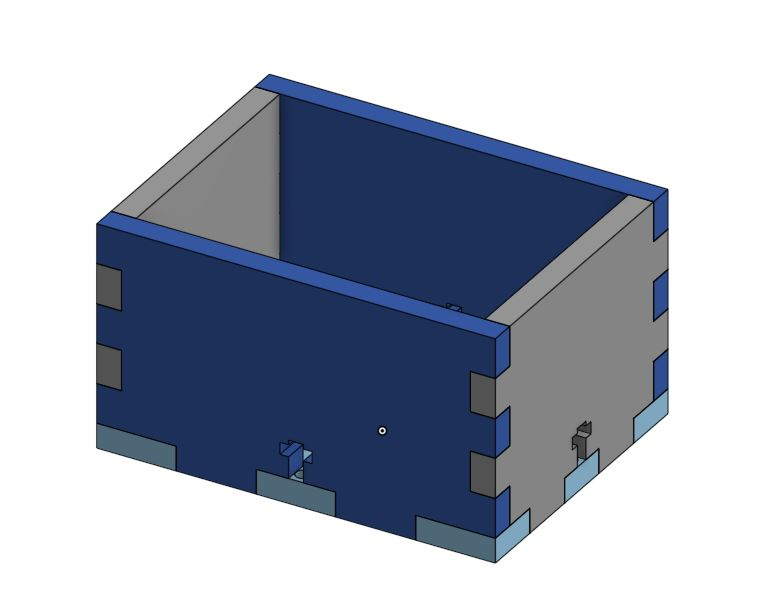
\includegraphics[width=0.95\textwidth]{Meetings/August/08-31-21/8-31-21_CAD_Image2 - Nathan Forrer.JPG}
  \caption{Five sided box}
  \label{fig:083121_2}
\end{minipage}
\end{figure}

\begin{figure}[htp]
\centering
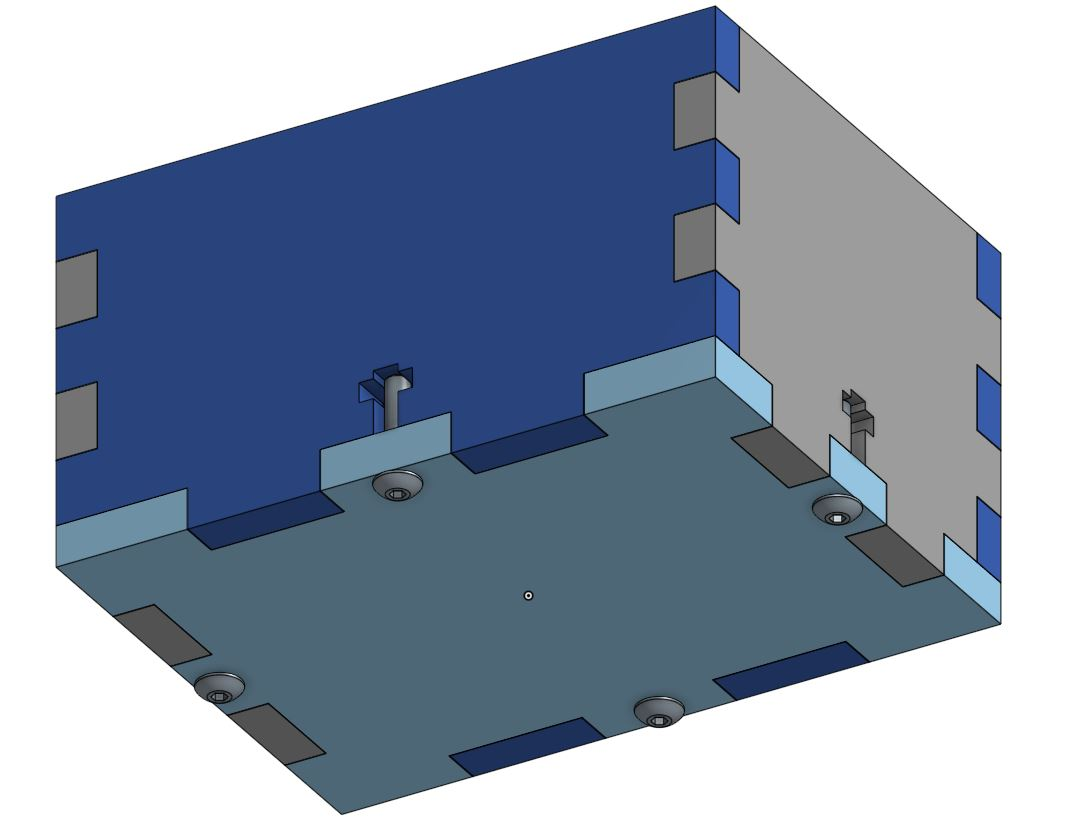
\includegraphics[width=0.95\textwidth, angle=0]{Meetings/August/08-31-21/8-31-21_CAD_Image3 - Nathan Forrer.JPG}
\caption{Inserting screws}
\label{fig:083121_3}
\end{figure}


\hhscommittee{Multimedia}
\noindent\hfil\rule{\textwidth}{.4pt}\hfil
\subsubsection*{Goals}
\begin{itemize}
    \item Today's goal for the Multimedia Committee was to make progress on the Team Takeover files.
  

\end{itemize} 

\noindent\hfil\rule{\textwidth}{.4pt}\hfil

\subsubsection*{Accomplishments}
Today, Falon and Rose worked on the Team Takeover Photoshop document. We spent the meeting adding new photos and editing them, as well as writing captions for each one. We have finished Jensen and Nathan's photos, but need photos for many of the other members. The Multimedia Committee will continue with this during the next meeting, and hopefully be able to finish more Team Takeover folders for members of our team.

\whatsnext{
\begin{itemize}
    \item Teach less experienced CAD members other types of mates
	\item Show how to make more complicated skeletons 
\end{itemize} 
}